% figures/fused-mixed-schedule.tex
% Fused mixed-policy schedule: one launch, four warp slots per
% block, then one CTA task per block, driven by task_ids.
\documentclass[tikz,border=10pt]{standalone}
% figures/common-preamble.tex
% Shared setup for the TikZ documentation figures. Colors mirror the
% palette in scripts/render_docs_diagrams.py so both atlases match.
\usepackage[T1]{fontenc}
\usepackage{lmodern}
\usepackage{tikz}
\usepackage{pgfplots}
\pgfplotsset{compat=1.18}
\usetikzlibrary{arrows.meta}
\usetikzlibrary{backgrounds}
\usetikzlibrary{calc}
\usetikzlibrary{decorations.pathreplacing}
\usetikzlibrary{fit}
\usetikzlibrary{positioning}

\definecolor{swcanvas}{HTML}{FFFDF8}
\definecolor{swpanel}{HTML}{F5F3ED}
\definecolor{swink}{HTML}{17212B}
\definecolor{swmuted}{HTML}{4B5563}
\definecolor{swline}{HTML}{59636E}
\definecolor{swblue}{HTML}{00689D}
\definecolor{swbluefill}{HTML}{DCEFFD}
\definecolor{swpurple}{HTML}{8E4775}
\definecolor{swpurplefill}{HTML}{F7E2EF}
\definecolor{sworange}{HTML}{A94500}
\definecolor{sworangefill}{HTML}{FCE5DC}
\definecolor{swgreen}{HTML}{00664B}
\definecolor{swgreenfill}{HTML}{DDF4EB}
\definecolor{swgrayfill}{HTML}{EEF0F2}

\pagecolor{swcanvas}
\AtBeginDocument{\color{swink}}

\tikzset{
  swcell/.style={
    draw, minimum width=0.46cm, minimum height=0.46cm, inner sep=0pt,
    line width=0.7pt, rounded corners=1pt},
  swbox/.style={
    draw=swline, fill=swpanel, rounded corners=6pt, line width=0.9pt},
  swarrow/.style={-{Stealth[length=6pt]}, draw=swline, line width=1pt},
  swtag/.style={
    draw, rounded corners=8pt, line width=0.9pt,
    font=\bfseries\scriptsize, inner xsep=8pt, inner ysep=4pt},
  swtitle/.style={anchor=west, font=\Large\bfseries, text=swink},
  swsubtitle/.style={anchor=west, font=\small, text=swmuted},
  swcode/.style={font=\small\ttfamily, text=swink},
  every picture/.style={line cap=round},
}

\begin{document}
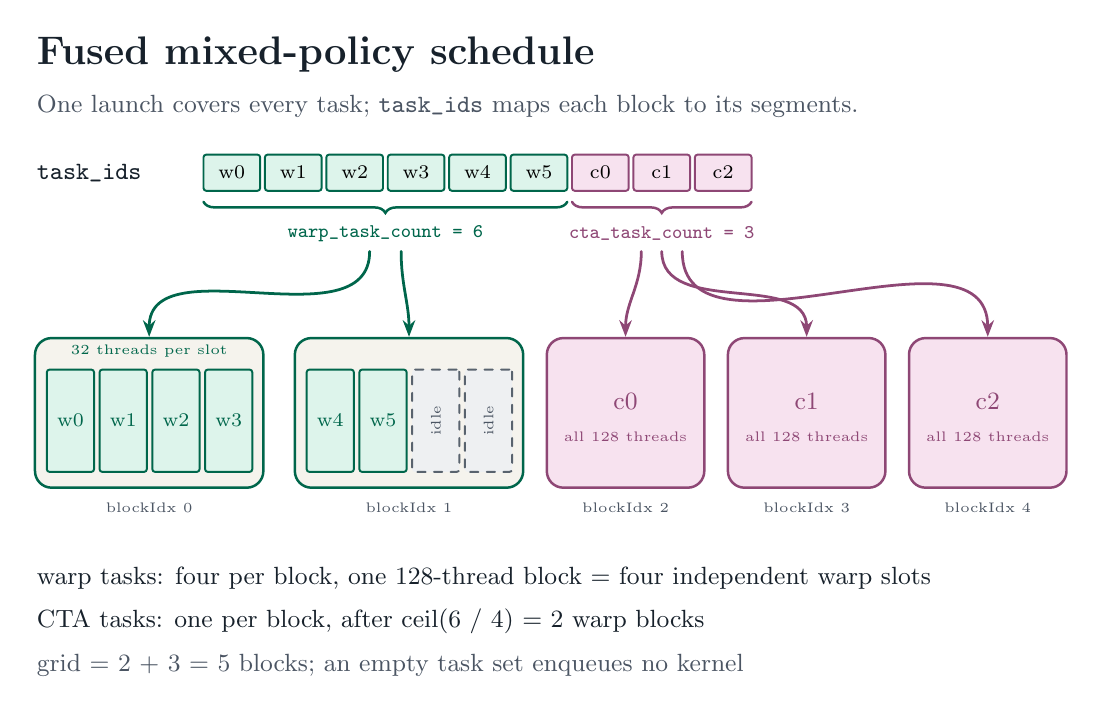
\begin{tikzpicture}[x=1cm, y=1cm]

% Header.
\node[swtitle] at (0, 1.15) {Fused mixed-policy schedule};
\node[swsubtitle] at (0, 0.5)
  {One launch covers every task; {\ttfamily\detokenize{task_ids}} maps
   each block to its segments.};

% Task list: warp tasks first, then CTA tasks.
\node[anchor=west, font=\small\ttfamily, text=swink] at (0, -0.35)
  {\detokenize{task_ids}};
\foreach \i/\lab in {0/w0, 1/w1, 2/w2, 3/w3, 4/w4, 5/w5} {
  \node[swcell, minimum width=0.72cm, fill=swgreenfill, draw=swgreen]
    (t\i) at (2.6 + \i * 0.78, -0.35) {\scriptsize\lab};
}
\foreach \i/\lab in {6/c0, 7/c1, 8/c2} {
  \node[swcell, minimum width=0.72cm, fill=swpurplefill, draw=swpurple]
    (t\i) at (2.6 + \i * 0.78, -0.35) {\scriptsize\lab};
}
\draw[decorate, decoration={brace, mirror, amplitude=4pt}, swgreen,
      line width=0.9pt] (2.24, -0.72) -- (6.86, -0.72);
\node[font=\scriptsize\ttfamily, text=swgreen] at (4.55, -1.12)
  {\detokenize{warp_task_count = 6}};
\draw[decorate, decoration={brace, mirror, amplitude=4pt}, swpurple,
      line width=0.9pt] (6.92, -0.72) -- (9.2, -0.72);
\node[font=\scriptsize\ttfamily, text=swpurple] at (8.06, -1.12)
  {\detokenize{cta_task_count = 3}};

% Grid of blocks: warp blocks carry four slots, CTA blocks carry one.
\foreach \b in {0, 1} {
  \node[swbox, draw=swgreen, minimum width=2.9cm, minimum height=1.9cm]
    (b\b) at (1.55 + \b * 3.3, -3.4) {};
  \node[font=\tiny, text=swmuted] at (1.55 + \b * 3.3, -4.6)
    {blockIdx \b};
}
\foreach \s in {0,...,3} {
  \node[swcell, minimum width=0.6cm, minimum height=1.3cm,
        fill=swgreenfill, draw=swgreen]
    (s0\s) at (0.55 + \s * 0.67, -3.5) {};
  \node[font=\scriptsize, text=swgreen] at (0.55 + \s * 0.67, -3.5)
    {w\s};
}
\foreach \s/\lab/\style in {0/w4/full, 1/w5/full} {
  \node[swcell, minimum width=0.6cm, minimum height=1.3cm,
        fill=swgreenfill, draw=swgreen]
    (s1\s) at (3.85 + \s * 0.67, -3.5) {};
  \node[font=\scriptsize, text=swgreen] at (3.85 + \s * 0.67, -3.5)
    {\lab};
}
\foreach \s in {2, 3} {
  \node[swcell, minimum width=0.6cm, minimum height=1.3cm,
        fill=swgrayfill, draw=swline, dashed]
    (s1\s) at (3.85 + \s * 0.67, -3.5) {};
  \node[font=\tiny, text=swmuted, rotate=90]
    at (3.85 + \s * 0.67, -3.5) {idle};
}
\node[font=\tiny, text=swgreen] at (1.55, -2.62)
  {32 threads per slot};
\foreach \b/\lab in {0/c0, 1/c1, 2/c2} {
  \node[swbox, draw=swpurple, fill=swpurplefill, minimum width=2.0cm,
        minimum height=1.9cm] (c\b) at (7.6 + \b * 2.3, -3.4) {};
  \node[font=\small, text=swpurple] at (7.6 + \b * 2.3, -3.25) {\lab};
  \node[font=\tiny, text=swpurple] at (7.6 + \b * 2.3, -3.7)
    {all 128 threads};
  \node[font=\tiny, text=swmuted] at (7.6 + \b * 2.3, -4.6)
    {blockIdx \pgfmathparse{int(2 + \b)}\pgfmathresult};
}

% Task-to-block routing, fanning out below the count labels.
\draw[swarrow, draw=swgreen] (4.35, -1.35) to[out=-90, in=90]
  (b0.north);
\draw[swarrow, draw=swgreen] (4.75, -1.35) to[out=-90, in=90]
  (b1.north);
\draw[swarrow, draw=swpurple] (7.8, -1.35) to[out=-90, in=90]
  (c0.north);
\draw[swarrow, draw=swpurple] (8.06, -1.35) to[out=-90, in=90]
  (c1.north);
\draw[swarrow, draw=swpurple] (8.32, -1.35) to[out=-90, in=90]
  (c2.north);

% Reading of the schedule.
\node[anchor=west, font=\small, text=swink] at (0, -5.5)
  {warp tasks: four per block,
   one 128-thread block = four independent warp slots};
\node[anchor=west, font=\small, text=swink] at (0, -6.05)
  {CTA tasks: one per block, after ceil(6 / 4) = 2 warp blocks};
\node[anchor=west, font=\small, text=swmuted] at (0, -6.6)
  {grid = 2 + 3 = 5 blocks; an empty task set enqueues no kernel};

\end{tikzpicture}
\end{document}
